% file: decision-tree-model.tex

\documentclass{standalone}
\usepackage{tikz}
\usepackage{tikz-qtree}
\usetikzlibrary{shapes}

\begin{document}
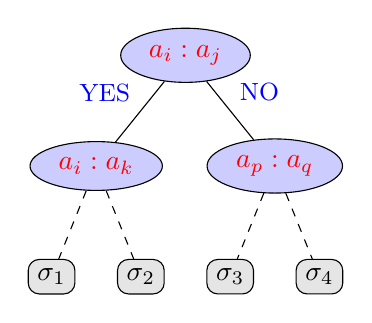
\begin{tikzpicture}[level distance = 40pt, sibling distance = 15pt,
  edge from parent/.style= { % added code
      draw, edge from parent path = {(\tikzparentnode) -- (\tikzchildnode)}},
  leaf/.style = {rectangle, rounded corners, fill = lightgray!40}]
  \tikzset{every tree node/.style = 
    {align = center, ellipse, draw, fill = blue!20}}

    \Tree [.{\textcolor{red}{$a_i : a_j$}}
	\edge node[auto = right]{\textcolor{blue}{\small YES}}; [.{\textcolor{red}{$a_i : a_k$}}
	    \edge[dashed]{}; [.\node[leaf]{$\sigma_1$}; ]
	    \edge[dashed]{}; [.\node[leaf]{$\sigma_2$}; ]
	  ]
	  \edge node[auto = left]{\textcolor{blue}{\small NO}}; [.{\textcolor{red}{$a_p : a_q$}}
	    \edge[dashed]{}; [.\node[leaf]{$\sigma_3$}; ]
	    \edge[dashed]{}; [.\node[leaf]{$\sigma_4$}; ]
	  ] 
	]
  \end{tikzpicture}
\end{document}

